% RSI paper template

% This is main.tex

% DO NOT MODIFY this file, except to 
%  1. Add additional packages or
%  2. Add macros,
% if you know what you are doing or are following directions of one of
% the technical staff.

\RequirePackage[2020-02-02]{latexrelease}
\documentclass[12pt,titlepage]{article}
\usepackage{rsipacks}


\usepackage[utf8]{inputenc}
\usepackage{float}
%\usepackage[english]{babel}
%% If you need to define macros or include more packages, do all that here.
%% Otherwise leave this file alone.  DO NOT type your paper text in here.

\usepackage{color,colortbl}

\setcounter{secnumdepth}{3}

\theoremstyle{plain}
\newtheorem{theorem}{Theorem}
\newtheorem{corollary}[theorem]{Corollary}
\newtheorem{lemma}[theorem]{Lemma}
\newtheorem{proposition}[theorem]{Proposition}
\newtheorem{conjecture}[theorem]{Conjecture}
\newtheorem{claim}[theorem]{Claim}

\theoremstyle{definition}
\newtheorem{definition}[theorem]{Definition}
\newtheorem{example}[theorem]{Example}

\theoremstyle{remark}
\newtheorem{remark}[theorem]{Remark}

\crefname{claim}{claim}{claims}
\Crefname{claim}{Claim}{Claims}
\crefname{app-corollary}{corollary}{corollaries}
\Crefname{app-corollary}{Corollary}{Corollaries}
\crefname{app-definition}{definition}{definitions}
\Crefname{app-definition}{Definition}{Definitions}
\crefname{figure}{figure}{figures}
\Crefname{figure}{Figure}{Figures}
\crefname{lemma}{lemma}{lemmata}
\Crefname{lemma}{Lemma}{Lemmata}
\crefname{app-lemma}{lemma}{lemmata}
\Crefname{app-lemma}{Lemma}{Lemmata}
\crefname{app-proposition}{proposition}{proposition}
\Crefname{app-proposition}{Proposition}{Proposition}
\crefname{app-theorem}{theorem}{theorems}
\Crefname{app-theorem}{Theorem}{Theorems}
\newcommand{\creflastconjunction}{, and~} %Implments the Oxford comma for non-compressed lists in \cref
\newcommand{\crefrangeconjunction}{--} %Implements n-dash for compressed lists in \cref
\doublespacing

\begin{document}

\setlength{\abovedisplayskip}{0pt}
\setlength{\belowdisplayskip}{0pt}
\setlength{\abovedisplayshortskip}{0pt}
\setlength{\belowdisplayshortskip}{0pt}

% This is cover.tex

% Insert your information as appropriate.

\title{A Rapid-Raman Spectroscopy and Machine Learning Based Approach for \textit{S. aureus} Detection in Milk}

\author{
Arjun Rao
\vspace{0.5in}\\
Under the direction of\\
\\
Utpal Tatu\\
Professor, Department of Biochemistry\\
The Indian Institue of Science\\
\vspace{1in}
}

\date{
Research Science Initiative India\\
\rsifinalpaperdate
}


\begin{singlespace}
\maketitle
\end{singlespace}

\begin{abstract}
\begin{singlespace}
% This is abstract.tex

This study proposes a novel pipeline for rapidly detecting \textit{S. aureus} in milk samples using Raman spectroscopy and machine learning. In utilizing a two-pronged approach for optimizing accuracy using Principal Component Analysis and ensuring maximum interpretability using Shapely Activated exPlanations (SHAP) analysis. Most of the models achieved above 90\% AUROC, demonstrating proof of concept using the smaller 55 spectra dataset obtained. This pipeline for quality control offers a rapid, 10-minute, cost-effective, and scalable method that can be implemented in dairy processing centers with further study.

 
\end{singlespace}
\vspace{1in}
\begin{center}\textbf{Summary}\end{center}
\begin{singlespace}
% This is summary.tex

The presence of bacteria in milk varies the chemical composition of a milk sample, which can be detected using spectroscopic methods like Raman spectroscopy. Employing the power of predictive modelling to this use case of differentiating between bacterial and non-bacterial spectra has valuable contributions in quality control in milk samples. This study on using Raman spectroscopy and machine learning for detecting \textit{S. aureus} bacteria in milk not only focuses on producing maximum accuracy in the binary classification task but also aims to attribute individual predictions to specific features in the spectra, thus enhancing interpretability. This pipeline, overall, produces an easily discernible, fast, cost-effective, and scalable method for detecting bacterial contamination in milk. 
\end{singlespace}
\end{abstract}

% This is paper.tex

\section{Introduction}
\textit{Staphylococcus aureus} is a common human pathogen that is responsible for, among other infections, bacteremia and food poisoning, especially in non-industrialized and newly industrialized regions \cite{Tong2015}. \textit{S. aureus} produces 18 enterotoxins, some of which are heat-resistant proteins, which may persist in milk after pasteurization \cite{SciDir_SD_StaphEnterotoxin, Jin2016}. \textit{S. aureus} is commonly present in milk, which is backed up by data from Brazil, which reveals that the presence of the bacteria in raw milk is 46\% and in pasteurized milk is 6.12\%. This underscores the need for rapid, accurate detection of \textit{S. aureus} in milk \cite{Zhang2023}. Raman spectroscopy can be used along with chemometric analysis to achieve this level of precise analysis, at a component by component basis, by utilizing the characteristic Raman shift taking place during Raman or inelastic scattering of particles for a particular bond.\\

\noindent The advantage conferred by using Raman spectroscopy for this particular study over the more conventional Fourier transform infrared spectroscopy (FTIR) is that sample preparation is significantly easier. Infrared waves are absorbed by an aqueous medium, making it difficult to analyze substances like milk. Raman scattering overcomes this issue, enabling easier and faster extraction of the chemical compositions of liquids like milk samples \cite{AzoOptics_1291}. Additionally, Raman spectroscopy offers greater spatial resolution and is sensitive to some bonds that are infrared-inactive \cite{Walzak_FTIR_Raman}. \\

\noindent The choice of selecting \textit{S. aureus} as a bacterium for this study is motivated by its role in bovine mastitis, its prevalence in milk samples and its part in causing food poisoning. Mastitis is an inflammation of the mammary gland due to, among other factors, microorganism infection, causing an increase in the somatic cell count in the infected cow’s milk \cite{Buczacki2020}. \textit{S. aureus} is a leading cause of bovine mastitis, as the bacteria live in the mammary gland epithelial cells and interact with the host cells, promoting bacterial adhesion and invasion \cite{Pavlova2022}. Thus, employing Raman spectroscopy and predictive models for \textit{S. aureus} detection can also help in early detection of some cases of bovine mastitis. \\

\noindent Existing literature on the subject, which uses predictive models and Raman spectroscopy, uses it for classifying bacteria in an aqueous or meat sample and uses simpler models like partial least squares regression \cite{Klein2023,Smith2024}. That being said, deep learning is increasingly becoming popular for bacterial classification using Raman spectroscopy and has also been used to differentiate between methicillin-resistant and susceptible \textit{S. aureus} strains; these studies feature very large sample sizes \cite{Ho2019}. The use of specific Machine Learning (ML) models, like the Gaussian process classifier and Naive Bayes Classifier, which can be trained on a smaller sample, and its ability to detect bacteria have not been fully investigated. The usage of this pipeline in milk samples on the target bacteria has only been used to identify enterotoxin B and not the bacteria itself \cite{DoeJRS6296}. \\

\noindent The regular method used by such models involves dimensionality reduction techniques like principal component analysis followed by machine or deep learning models. Other methods aim to extract features such as peak intensity from the Raman spectra, but these two methods haven’t effectively been compared in the context of specific bacterial prediction. It is also worth pointing out that analysis for bacterial prediction uses surface-enhanced Raman spectroscopy, which uses metal nanoparticles to improve the sensitivity of the Raman spectra, thus making detection using these methods more complicated and costly \cite{DoeJRS6296}. \\

\noindent This study hypothesizes that Raman spectroscopy, in combination with classical and probabilistic ML classifiers, can accurately distinguish \textit{S. aureus}-infected milk samples from uninfected controls, even under varying physicochemical conditions.


\section{ Technical Background} \label{sec:setting}

\subsection{Raman Spectroscopy}

Raman scattering is analogous to the more common Rayleigh scattering, in which light waves deviate from their straight path on interacting with suspended particles or molecules. In Rayleigh scattering, the light energy is scattered back at the same frequency as that of the incident light without interacting with the molecules. However, in Raman scattering, the photons interact with the electron clouds of the molecules, causing a change in the vibrational modes of the molecules. This change in vibration leads to a difference in the polarizability of the electron cloud \cite{SciHub76e3755}. \\

\noindent Polarizability can be defined as the ease with which the electron cloud can be distorted by an external electric field. For highly polar molecules, there is a minimal change in the polarizability of the compounds, and this derivative of polarizability corresponds to energy shift in inelastic or Raman scattering. The energy shifts itself occur due to a decrease in energy in the photons scattered when the molecule returns from the excited vibrational mode to the regular mode. The energy dispersed during Raman scattering is defined as the scattering intensity and is proportional to the square of the change in the induced dipole forces \cite{TracesLab_RamanUnderstanding}. This shift in energy during inelastic scattering can be related to a proportional shift in frequency and wavelength by the Planck relation in \autoref{eq:1} \cite{EnergyWaveTheory_Ehf}. \\
\begin{equation}
\label{eq:1}
E = hf = h\frac{c}{\lambda} 
\end{equation}
 \\
\noindent Raman spectroscopy utilizes this characteristic shift in the frequency and intensity of scattering for fingerprinting particular bonds in a molecule for identification. The characteristic frequency shift that enables the detection of the molecule is given by the formula given below, which relates the idea of the energy shift with the Planck relation as seen in \autoref{eq:2}\cite{Berciu_Phys502_Raman}. \\
\begin{equation}
\label{eq:2}
v_s = |v - \frac{\Delta E}{h}| 
\end{equation} \\
\noindent The modulus in the above formula can be explained by the presence of Stokes and anti-Stokes scattering. In Stokes scattering (which occurs for $1$ in $10^7$ photons), the photon released has less energy than the incident photon, as the molecules release them on reverting to the ground state from a high-energy state. This is in contrast to the rarer anti-Stokes scattering, in which the scattered photon is at a higher energy than the incident photons \cite{DoITPoMS_StokesStokes}. \\

\noindent A Raman spectroscope makes use of this principle to detect the chemical composition of a sample by measuring the Raman shift in the photons of the high-intensity laser undergoing inelastic scattering due to the sample. Thus, it provides a non-destructive and easy-to-use method to detect chemical variation in milk samples due to bacterial presence.

\subsection{Principal Component Analysis and Predictive Models}

Principal Component Analysis (PCA) is a statistical technique that reduces the number of features while preserving the relations between the input variables. This is typically used for a high-dimensionality dataset like the output data of the Raman spectrometer \cite{Greenacre2022PCA}. This process involves selecting the eigenvectors corresponding to the greatest eigenvalues of the covariance matrix of the input matrix \cite{Shalizi2022Ch18}. Additionally, reducing the number of dimensions enables greater analysis of data and ensures the provision of generalizable trends in variance without overfitting, which can occur in alternative methods like Partial Least Squared Discriminant Analysis (PLS-DA) \cite{Woodgate2016RSTA}. In the context of Raman spectroscopy, it can also be used to reduce fluorescent background by preserving features with high statistical relevance. \\ 

\begin{figure}
    \centering
    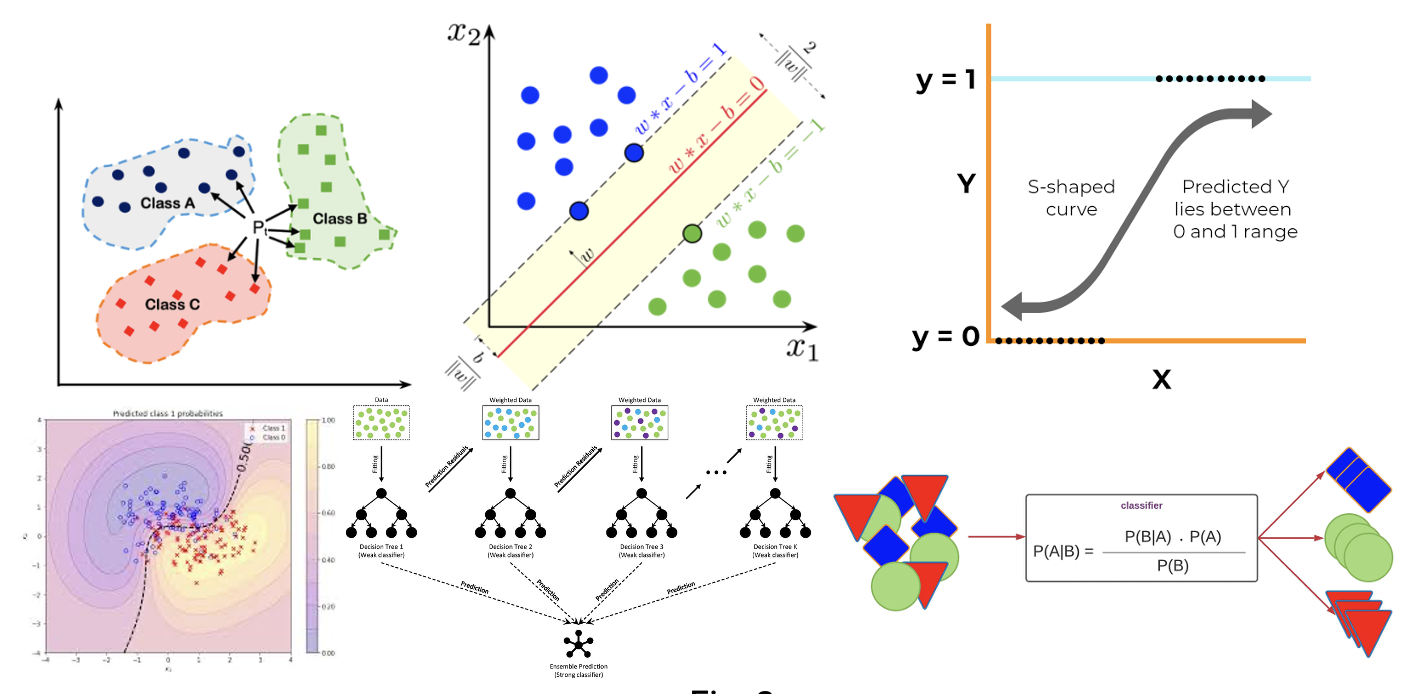
\includegraphics[width=0.8\linewidth]{Figures/Model_Architecture.png}
    \caption{Architecture of ML Models used: 1) K-Nearest Neighbor \cite{imageknn}, 2) Support Vector Machine \cite{Singh2025_SupervisedLearningCheatSheet}, 3) Logistic Regression \cite{DataLensBlogger2024_ClassificationCheatSheet} , 4) Gaussian Process Classifier \cite{Kulkarni2024_Day10SLA3} , 5) Random Forest Classifier \cite{ranforest} , 6) Naive Bayes Classifier \cite{MLArchive_NaiveBayes2023} }
    \label{fig:model-architecture}
\end{figure}


\noindent After performing PCA and requisite data analysis, the data becomes ready to be trained. Given that this study involves a binary classification task and has a small training set, the choice of models must ensure that the models do not overfit and are able to generalize well. Logistic regression is a discriminant model that predicts the probability of the given data belonging to a particular class and uses a threshold value for classifying the data. Due to its interpretability and ability to provide prediction probabilities, logistic regression is a good option \cite{JurafskySLP3_Ch5}. In contrast to logistic regression, the Naive Bayes classifier uses conditional probability for classification and provides a high accuracy on smaller datasets \cite{Anonymous2012NaiveBayesRG}. \\

\noindent Gaussian Process Classifiers (GPCs) use a probabilistic model to classify an input based on its attributes using the Gaussian Process. This is a stochastic model that assigns probabilities to various functions that model the distribution of the training data \cite{Goertler2019DistillGP}. Being a probabilistic model, GPCs can perform well for small datasets. Support Vector Machines and K-Nearest Neighbor Classifiers aim to create a boundary between the two classes by creating a hyperplane or determining it based on the attributes of the neighbor \cite{MITSVM,SciDirectKNN}. Tree-based models involve an information gain at each node and make predictions based on the classification at each node. These models can generalize well for small and large datasets. The two tree-based models that have a simple architecture are the decision tree classifier and the random forest classifier, with the former consisting of one tree graph and the latter being made up of multiple decision trees \cite{MediumTreeML}. \\ 

\noindent \autoref{fig:model-architecture} represents the architecture of the models that are being used in this study for bacterial prediction. These model architectures enable learning from smaller samples and makes them ideal for predictive modeling for this task.

\section{Methodology} \label{sec:desc}

\subsection{Data Collection}

For this study, $n=55$ spectra were collected, of which 46 comprised the control, in which bacteria weren’t inoculated, and the remaining 9 were inoculated with two different concentrations of bacteria in the range $10^5 CFU/mL$ to $10^6 CFU/mL$. The strain of bacteria used was methicillin-resistant \textit{S. aureus}, which was incubated in LB agar medium for 16 hours at 250 rpm and 37°C. The proximal concentrations were reached after diluting the initial concentration determined using spectrophotometry at OD600 (initial value obtained in this study was 0.640) \cite{Yang2013_srep01863}.  For the control sample, physical conditions like pH and temperature and milk type were varied, as can be seen in Table 1A. The bacterial concentration range was chosen as it's the average bacterial load in mastitic cows and is the bacterial concentration regularly found in contaminated milk \cite{doVale2023mastitis}. The LabRam HR Evol Raman spectroscope by HORIBA Scientific was used to collect the data with a 532 and 514 nm laser for 10 accumulations each with an acquisition time of 10 seconds in the spectral range $400-3500 cm^{-1}$. 

\subsection{Data Augmentation}

Due to an imbalance in the class size between the control group and the experimental group, data augmentation is needed to create a greater number of samples in the experimental group. This can be done by adding random Gaussian noise to the intensities in the experimental group, thus increasing the number of samples while also simulating changing bacterial concentration \cite{CEA_HAL_01839859}. The output of such a function, which adds noise for generalization, is given in \autoref{eq3}. \\
\begin{equation}
\label{eq3}
x = s + \psi
\end{equation} \\
\noindent Where $x$ is the output value, which takes in $s$, the true value, and $\psi$, which represents the additive white noise produced by a normal distribution function \cite{SciDirect_WhiteNoise}. For this study, data augmentation was primarily performed for the experimental sample, and the total number of spectra was increased to 94 samples. Later analysis, also reveals insignificant variation in Raman Spectra caused by varying physical conditions, thus justifying the use of data augmentation to introduce arbitrary spectral variation. 

\subsection{Data Pre-processing and Baseline Correction}

After obtaining the spectra, smoothing was performed using the Savitsky-Golay filter to denoise the spectral data. This method, commonly used in chemometrics, involves minimizing the least squared loss between a certain polynomial function selected for a particular window size.  For this particular data, the window size selected was 5, and a quadratic order was selected \cite{SciHub_AC60214a047}. Denoising helps machine learning models better learn the generic features as opposed to specific features. \\

\begin{figure}
    \centering
    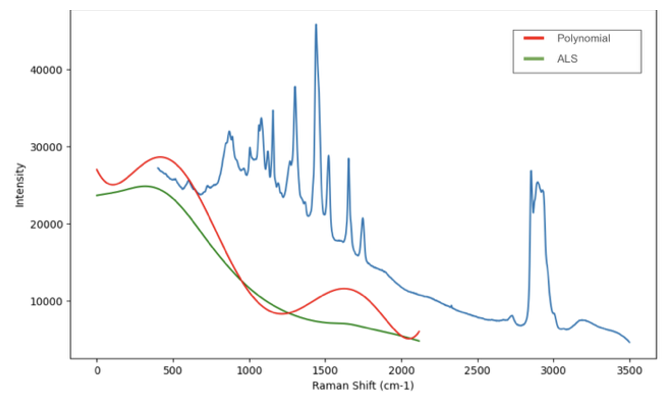
\includegraphics[scale=0.8]{Figures/ALSvPoly.png}
    \caption{Comparing ALS with Polynomial Regression for Baseline Fitting. ALS shows greater ability in modeling fluorescence noise.}
    \label{fig:baseline-fit}
\end{figure}

\noindent After denoising, baseline correction was used to correct for the fluorescence background in the Raman spectra. Fluorescence occurs due to background light interfering with the Raman signals \cite{Cebeci2017_FluorescenceBackground}. This background elevates the baseline of the Raman spectrum and may obscure weak signals. This can be corrected by statistical techniques to subtract the background signal, using baseline correction. For an arbitrary Raman spectrum, the asymmetric least squares method was compared against polynomial fitting to determine the optimal method for baseline correction. \autoref{fig:baseline-fit} represents the comparative performance of ALS (with a threshold of 0.01, asymmetric value of $10^6$, and 10 iterations) and the Polynomial Fitting Model ($7^{th}$ degree.)  The baseline established by the ALS model does not overfit to the spectral curve and prevents the spectra from having negative intensities; thus it was used for baseline correction. \\

\noindent Exploratory Data analysis was performed on this processed data; however, for training machine learning models, normalization is needed to standardize the ranges of the features being considered. $l^2$ normalization involves using the Euclidean Normal to preserve the direction of a vector while scaling down the magnitude of the vector. \cite{Celebi2010_EuclideanNormApprox} This also helps to prevent overfitting and to ensure that the model is able to generalize well. 

\subsection{Exploratory Data Analysis}

After extrapolating data that can be used for analysis after performing baseline correction and denoising, the control data was analyzed to examine the effect of changing conditions on the Raman spectra of milk samples. The control group was isolated for this analysis due to the absence of variation in spectra due to the presence of bacteria. Analysis of the average spectra of toned milk and comparing that with full-cream milk indicates the greatest difference at the lipid sections of the spectra at 1416, 2865, and 2902 $cm^{-1}$, which shows on the spectra the lower fat percentage in toned milk compared to full cream, as can be seen in \autoref{fig: tonedfc}. This can be further validated by performing a PCA analysis at 3 dimensions, which shows the ability to divide the toned and full-cream samples using a plane. While there are some outliers, there appears to be a distinct discriminative separation pattern created in \autoref{fig:pcatonedfc}. \\

\begin{figure}[htbp]
  \centering
  \begin{subfigure}[b]{0.45\textwidth}
    \centering
    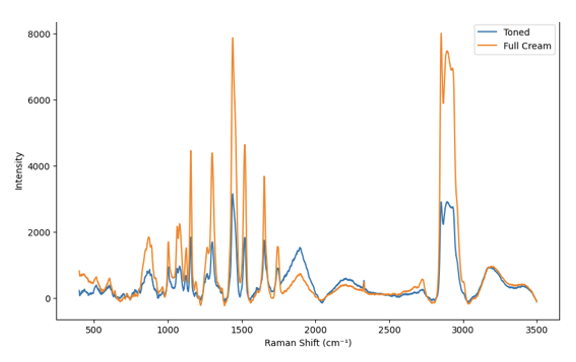
\includegraphics[scale=0.5]{Figures/TonedFC.png}
    \caption{Raman Spectra of Toned and Full Creme Milk representing variation in fat content.}
    \label{fig: tonedfc}
  \end{subfigure}
  \hfill
  \begin{subfigure}[b]{0.45\textwidth}
    \centering
    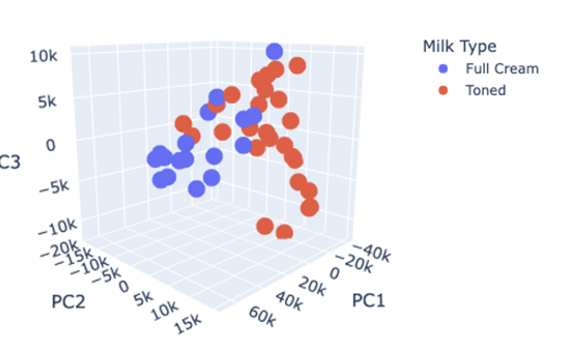
\includegraphics[scale=0.5]{Figures/PCA_tonedFC.png}
    \caption{PCA Analysis of Types of Milk indicating differentiability in Raman Spectra.}
    \label{fig:pcatonedfc}
  \end{subfigure}
  \caption{Comparison of  Toned and Full Creme Milk.}
  \label{fig:combined2}
\end{figure}

\noindent The other physical conditions that were varied in the control group, did not contribute to significant variation in the Raman Shifts as seen in Appendix A. Therefore, this fact justifies not varying physical factors for the bacterial sample and only analyzing the variation in bacterial concentration. \\

\noindent The analysis of the Raman spectra of milk samples containing and not containing \textit{S. aureus} were analyzed using similar metrics of a direct comparison in the spectra along with the changes in PCA it translated to, as seen in \autoref{fig:combined}. Analysis of the spectra created from the mean intensities reveals that the spectra with the bacterial sample consists of a greater number of peaks compared to the control sample. This is attributable to the proteins and other components present in the bacteria itself. Further, bacterial presence also suppresses the Raman peaks of milk, especially in the region between 1000 and 2000 $cm^{-1}$ corresponding to some of the protein and fatty acid peaks. Comparing the spectra obtained with the known spectral peaks for \textit{S. aureus} can lead to possible classifications. The peaks at 1160 and 700-800 $cm^{-1}$ can be attributed to the presence of carotenoids and nucleic acids, respectively \cite{Liu2025_RamanSingleCell}. The region between 1800-2800 $cm^{-1}$ is typically referred to as the silent region of the Raman spectra; however, in the spectra in \autoref{fig:bacteria}, there are a large number of minor peaks. These can be attributable to shifts in the original peaks of the milk proteins due to bacterial action on the milk proteins. Proteins like casein can show structural rearrangement, causing a shift in the position of the amide groups \cite{Movasaghi2007}. The major peaks at 2150 and 1900 $cm^{-1}$ can also be attributed to possible impurities that lead to unexplainable peaks in the Raman spectra. A decrease in the relative intensity of the fatty acid peaks can also be noticed in the bacterial sample, which can be attributed to bacterial action decomposing fatty acids using beta-oxidation \cite{Kuiack2023_fadXDEBA}. This is further validated by peaks at 1450 and 724 $cm^{-1}$, indicating the presence of Acetyl-CoA, which is the product of beta oxidation of fatty acids \cite{Wang2023_RiP_SERS_DeepOcean}. \\

\begin{figure}[htbp]
  \centering
  \begin{subfigure}[b]{0.32\textwidth}
    \centering
    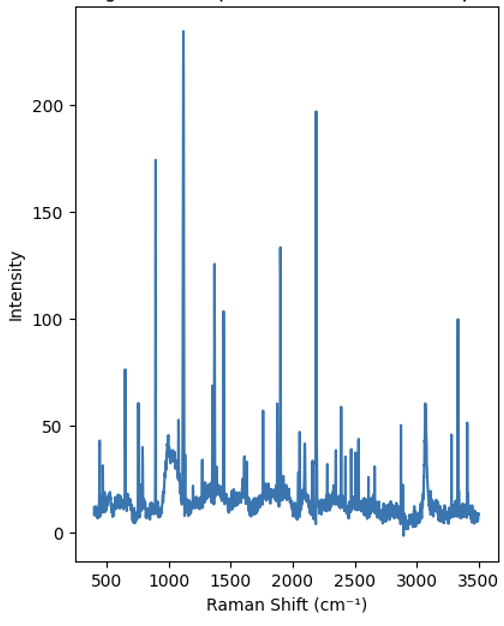
\includegraphics[width=\linewidth]{Figures/bacteria.png}
    \caption{Mean Intensities of Milk Samples inoculated with bacteria}
    \label{fig:bacteria}
  \end{subfigure}
  \hfill
  \begin{subfigure}[b]{0.32\textwidth}
    \centering
    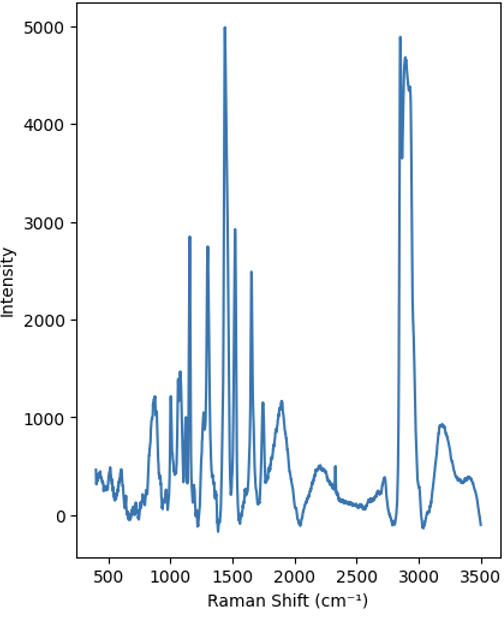
\includegraphics[width=\linewidth]{Figures/nonbacteria.png}
    \caption{Mean Intensities of Milk Samples not inoculated with bacteria}
    \label{fig:nobacteria}
  \end{subfigure}
  \hfill
  \begin{subfigure}[b]{0.32\textwidth}
    \centering
    \raisebox{1.5cm}{ % adjust the vertical offset as needed
      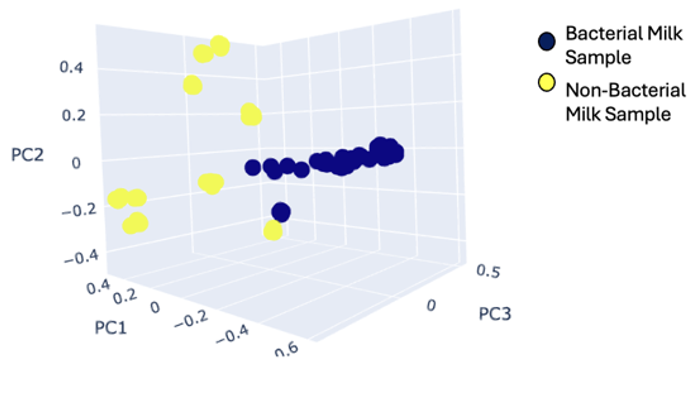
\includegraphics[height=3.5cm]{Figures/Screenshot 2025-07-16 at 2.27.37 PM.png}
    }
    \caption{PCA Analysis of Bacterial and Non-bacterial Sample}
    \label{fig:pcabac}
  \end{subfigure}
  \caption{Comparison of Raman spectra for Bacterial and Non-Bacterial Milk Samples indicates a difference in the number of constituents in the two groups.}
  \label{fig:combined}
\end{figure}




\noindent A PCA analysis of the given data, after performing normalization, shows a distinct separation that can be achieved between the points, samples with bacteria and without bacteria, by plotting a plane, enabling greater accuracy as seen in \autoref{fig:pcabac}. This data analysis serves as a basis for interpreting and extracting patterns in the predictions made by machine learning models. 

\subsection{Feature Extraction and Model Training }

This study, in using machine learning techniques, employs two separate pipelines for training models: 1) It directly trains the models on PCA-transformed data, and 2) it extracts features from the Raman spectra and trains the models on these features. The primary advantage conferred by the second approach over the first approach is that it enables model interpretability tests, thus reducing the perceived randomness in machine predictions. For both the pipelines, the following machine learning models were trained: 1) Gaussian Process Classifiers, 2) Random Forest Classifiers, 3) Gaussian Naive Bayes Classifiers, 4) K-Nearest Neighbors Classifier, 5) Support Vector Classifiers, and 6) Logistic Regression. The fact that these models use traditional and probabilistic methods enables them to learn and be tested on a smaller data sample. For the PCA-transformed data, stratified K-fold cross-validation with 5 folds was used to test predictive accuracy across various balanced test samples. \\

\noindent To compile the feature-extracted dataset, the following spectral variables were considered: 1) Area under curve, 2) Mean Peak Sharpness, 3) Number of Peaks, 4) Maximum Peak Sharpness, 5) Skewness of Peaks, and 6) Position of Maximum Intensity Peak. The area under the peaks helps quantify the number of bonds and their relative concentrations in the sample. The mean peak sharpness and maximum peak sharpness determine the clarity of the signals present in the sample and that of the signal with maximum intensity, which is clearly a visual difference observed in the spectra of the bacterial and non-bacterial samples in \autoref{fig:combined}. The number of peaks is a distinctive chemometric marker due to the presence of a greater number of proteins and other elements in the milk sample inoculated with \textit{S. aureus}. The position of the maximum intensity peak determined the most prominent signal in the sample, which can serve as an important differentiator due to the denaturation of milk proteins and fatty acids in bacterial presence. Lastly, skewness serves as a quantifiable metric of asymmetry, which can be seen as a visual marker in \autoref{fig:combined}. \\

\noindent The exact procedure used to extract the said features from the Raman spectra is given in Algorithm \autoref{alg:feature_extraction} in Appendix A, which consists of the formulae for the mentioned quantifiable parameters. The compiled dataset obtained from these various defined parameters was used to train the same machine learning models. Using existing model interpretability metrics, like Shapely Additive Explanations (SHAP), on these predictive models can help better understand the rationale behind the decisions taken by the ML models. 

\section{Results}
\subsection{Model Evaluation}

Evaluation for models using the two pipelines was performed using accuracy, recall, precision, F-1 scores, and area under the receiver operating curve. \autoref{tab:classifier_metrics} summarizes the evaluation metrics for the various ML models trained. It can be observed that many of the accuracy, recall, precision, and F1 scores for many of the models have the exact values. This can be explained by the relatively small testing size and similar classification parameters being used by the models. Due to this factor, it is important to evaluate model accuracy along with AUROC (Area under Receiver Operating Curve) values. Therefore, the two conditional probability-based models, Naive Bayes Classifier and GPC, can be deemed the best for classification of bacterial milk samples using Raman spectroscopy. \\

\begin{table}[htbp]
\raggedright
\caption{Performance comparison of various classifiers}
\label{tab:classifier_metrics}
\resizebox{\textwidth}{!}{%
\begin{tabular}{lcccccc}
\hline
\textbf{Evaluation Metric} & \textbf{Naive Bayes} & \textbf{Logistic Reg.} & \textbf{SVM} & \textbf{KNN} & \textbf{Random Forest} & \textbf{GPC} \\
\hline
Accuracy   & 92.5 & 89.2 & 89.2 & 89.2 & 89.2 & 89.2 \\
Precision  & 92.9 & 92.9 & 92.9 & 92.9 & 92.9 & 92.9 \\
Recall     & 95.6 & 88.9 & 88.9 & 88.9 & 88.9 & 88.9 \\
F1 Score   & 93.2 & 88.0 & 88.0 & 88.0 & 88.0 & 88.0 \\
AUROC        & 95.0 & 94.4 & 91.8 & 88.8 & 86.0 & 97.5 \\
\hline
\end{tabular}
}
\end{table}


\noindent For the feature extraction-based pipeline, after normalization, the best accuracy was displayed by the K-Neighbors Classifier and the Random Forest Classifier. These two models had a 100\% accuracy and therefore a 1.0 AUROC value, which once again can be attributed to the small test sample. While this high accuracy is typically attributed to overfitting, in this case there is a high correlation between the target variable, the presence of bacteria, and the dependent variables, making it plausible for a machine to accurately learn the underlying logic without necessarily overfitting. 

\begin{figure}[htbp]
    \centering
    \begin{subfigure}[b]{0.48\textwidth}
        \centering
        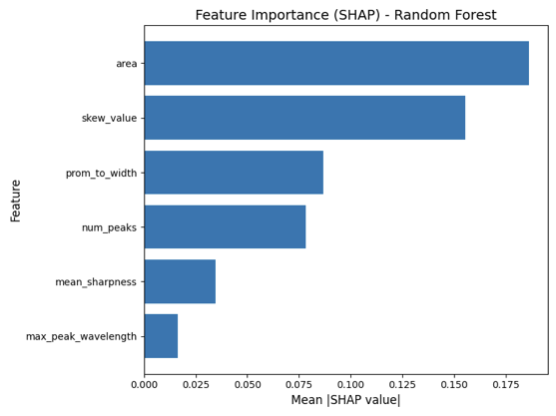
\includegraphics[width=\linewidth]{Figures/shap.png}
        \caption{Feature Importance for Random Forest Classifier. The analysis indicates greater importance for skewness and area under curve.}
        \label{fig:shap}
    \end{subfigure}
    \hfill
    \begin{subfigure}[b]{0.48\textwidth}
        \centering
        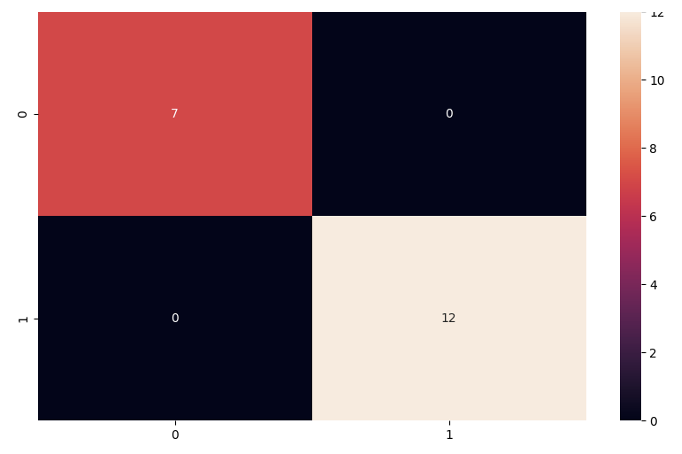
\includegraphics[width=\linewidth]{Figures/conf_matrix_rand forst.png}
        \caption{Confusion Matrix for K-Neighbor and Random Forest Classifiers.}
        \label{fig:cfbest}
    \end{subfigure}
    \caption{The Learning Parameters of the model are biochemically sound and highly precise.}
    \label{fig:shap_and_cf}
\end{figure}


\subsection{Model Interpretability}

SHapely Additive exPlanations (SHAP) is a unified framework used to determine feature importance, thus helping provide intuition to decisions taken by ML models \cite{LundbergLee2017_SHAP}. This method has been used for the feature-extracted dataset and the Random Forest Model, primarily due to its high accuracy and ease of interpretability compared to the K-Neighbors Classifier. In addition, it was validated that all models assigned similar relative importance to the features. \autoref{fig:shap} represents the results from this analysis, which reveals the greater importance being attached to the area under the spectra and the skewness of the graph. This can be further validated by a two-tailed t-test, the results of which are in Table 3A. \\

\noindent The bacterial sample was shown to have a greater number of peaks, leading to greater spectral asymmetry and higher skew. This represents an increase in the number of constituents. However, in comparing feature importance, the areas under the curve might have a disproportionately high importance due to difference in the arbitrary intensity units. Therefore, there is a need to better understand the actual relation between this feature and bacterial presence. The other features considered in this analysis and their respective feature importance can be considered a product of the number of peaks. 

\section{Discussion}

This study advances the current understanding of bacterial detection using a novel Raman spectroscopy with a machine learning pipeline. By using classical Raman spectroscopy and with detailed analysis of the interpretability of the machine learning models, this study provides data on how such a model can be used in an easy-to-use way in a real-life setting. That being said, it is important to recognize that this model was trained on samples of pasteurized milk. While post-pasteurization contamination is a plausible threat, especially in developing countries, \textit{S. aureus} and associated enterotoxins are more commonly found in raw milk. Raw milk consists of a greater number of pathogens, leading to greater spectral noise, making the detection of a particular type of bacteria more difficult \cite{Quigley2013_JDS4928}. Additionally, it is not clear whether classical Raman spectroscopy will be able to cut fluorescence noise in raw milk samples to a sufficient degree so as to be able to project the composition peaks clearly. \\

\noindent Due to the inability to access a single Raman spectroscope for an extended period of time, the control group was obtained using a 532 nm laser, while the bacterial sample was obtained using a 514 nm laser. While the calibration and instrument type were kept constant, the difference in the exact instrument creates an issue of a confounding variable. \autoref{fig:combined3} demonstrates the variation in spectra of the same milk type tested on the two different spectroscopes. While the position of the peaks is the same spectroscopically, differences in the peak sharpness and intensity can be observed. Some of these can be attributed to the fact that the batches of milk being compared are different; it is clear that the spectrum in \autoref{fig:sampath} are noisier as compared to the spectrum in \autoref{fig: horiba}. These instrumental variations also act as a stress test for the model to be able to learn from and be tested on spectroscopes, which are bound to have minor differences in calibration. \\

\noindent The sample size used for this particular study, of 55 real spectra, which was augmented to 94 samples, is small, and while it is sufficient to show proof-of-concept to build an industrial-grade detector using this pipeline, a larger sample size will be needed. Also, greater diversity in milk type and conditions will be needed to improve model generalization. A larger dataset also provides an opportunity to use deep learning techniques like convolutional neural networks (CNNs), which are likely to have greater predictive accuracy than traditional ML models. A larger study that draws on the baseline established in this study and expands the data size and corrects for instrumental variation will be an invaluable resource for the dairy industry in the rapid quality control of milk. 

\section{Conclusion} \label{sec:conclusion}

This study demonstrates conclusively the potential of a pipeline combining Raman spectroscopy and machine learning for detecting \textit{S. aureus} in milk samples. Achieving an AUROC of above 90\% for most of the models tested and being able to interpret the decisions taken by the model to a certain extent further validates the real-life applications of this model in not only bacterial prediction but also in early mastitis detection. The two-pronged approach of training ML models on PCA-transformed data and feature-extracted data creates a more robust pipeline for use cases in quality control. Conditional probability based models, in particular Naive Bayes Classifier showcased highly accurate and interpretable results in bacterial prediction, thus proving the initial hypothesis about the ability of such models to handle tasks involving classification with spectroscopic data. A similar pipeline to the one used in this study could also be used for a regression analysis to determine bacterial concentration in milk. A study that predicts the presence of multiple types of bacteria in milk samples will also be of great utility for the dairy industry. Future studies could also expand the scope of the study to not only predict bacterial presence but also predict mastitis based on somatic cell counts in milk, thus providing an end-to-end pipeline for milk quality control. This proposed method provides a faster method of detection than traditional ELISA or PCR-based tests, thus providing a scalable method for bacterial detection in milk. 


\section{Acknowledgments} 

I would like to thank Professor Utpal Tatu for providing access to his lab and for guiding the author through the entire process. I also wish to thank Dr. Vinay Bachu for providing constructive feedback at every stage of the writing process and Ms. Roohani Basavaraj, Ms. Gargi Dey, and Dr. H.C. Sudeeksha for providing technical support. The author would also like to express his gratitude towards the Sampath and HORIBA labs for providing access to the Raman spectroscopes. Additionally, I would like to offer my sincere gratitude to the Center for Excellence in Education, the Indian Institute of Science (IISc), and the entire RSI India staff for conducting the program with utmost professionalism. Lastly, he would like to specially thank the sponsors of the RSI India program, Dr. Sanjay Palsamudram and the Adani Group, for enabling access to the facilities at an institution of such prestige as IISc. 

\section{Code Access}

\noindent All code for this program including the data analysis, model training and interpretability is available publicly on GitHub. The programming language used for this study is Python (3.11.7) and additional specifications about the libraries used is available in the \texttt{requirements.txt} file in the GitHub repository. Additionally, the GitHub repository consists of the dataset and the saved models. The access link to the GitHub repository is as follows: https://github.com/arjun041008/RamanSpectroscopy.git








\begin{singlespace}
%\include{biblio}
\bibliographystyle{style.bst}

\bibliography{biblio}
\end{singlespace}

% This is appa.tex
%
% This file is for appendices.  If you don't have any appendices, delete
% the percent sign from the beginning of the next line.
%\endinput

\clearpage
\appendix
\section{Appendix: Figures and Tables}

\begin{figure}[h!]
    \centering
    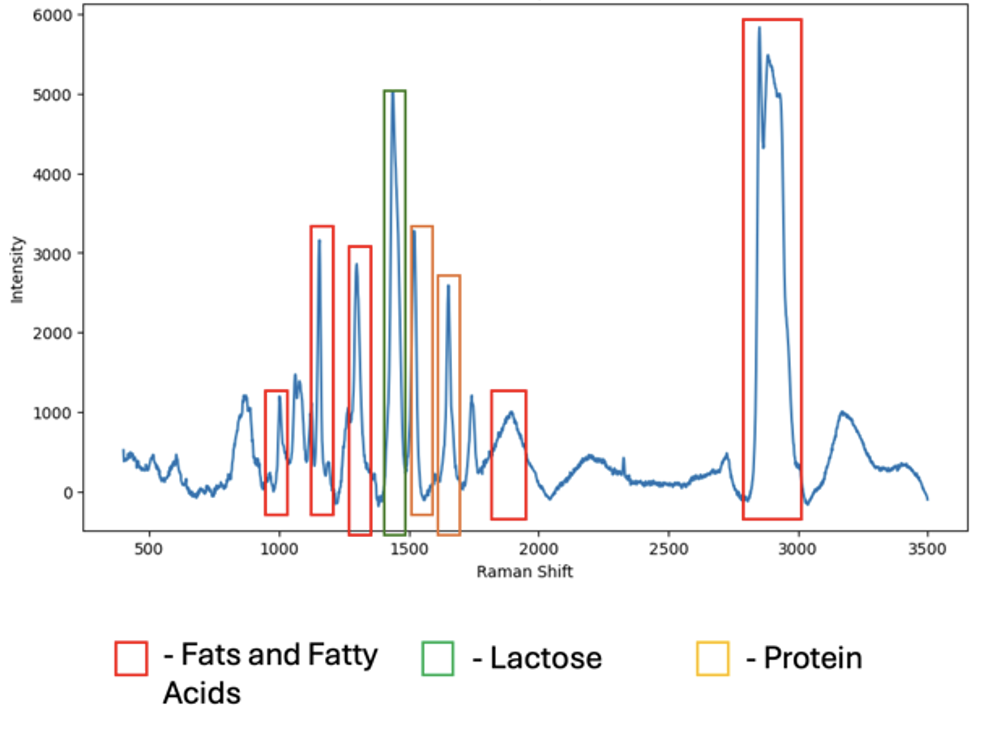
\includegraphics[width=0.5\linewidth]{Figures/Screenshot 2025-07-16 at 2.26.41 PM.png}
    \caption{Characterization of Raman Peaks for the Control Sample}
    \label{fig:ram}
\end{figure}

\begin{table}[h!]
\centering
\begin{tabular}{|l|c|l|}
\hline
\textbf{Functional Groups} & \textbf{Raman Band (cm\textsuperscript{-1})} & \textbf{Component} \\
\hline
Aromatic C--C & 1016 & Fat \\
CH\textsubscript{2} twist, Ester & 1279, 1315 & Fat \\
CH\textsubscript{2} bending & 1416, 1759 & Fat, Lactose \\
Amide I & 1566 & Proteins \\
Amide II & 1670 & Proteins \\
CH stretch & 2865, 2902 & Fatty Acids \\
\hline
\end{tabular}
\caption{Raman spectral bands of various functional groups in milk components}
\label{tab:raman_bands}
\end{table}


\begin{figure}[h!]
    \centering
    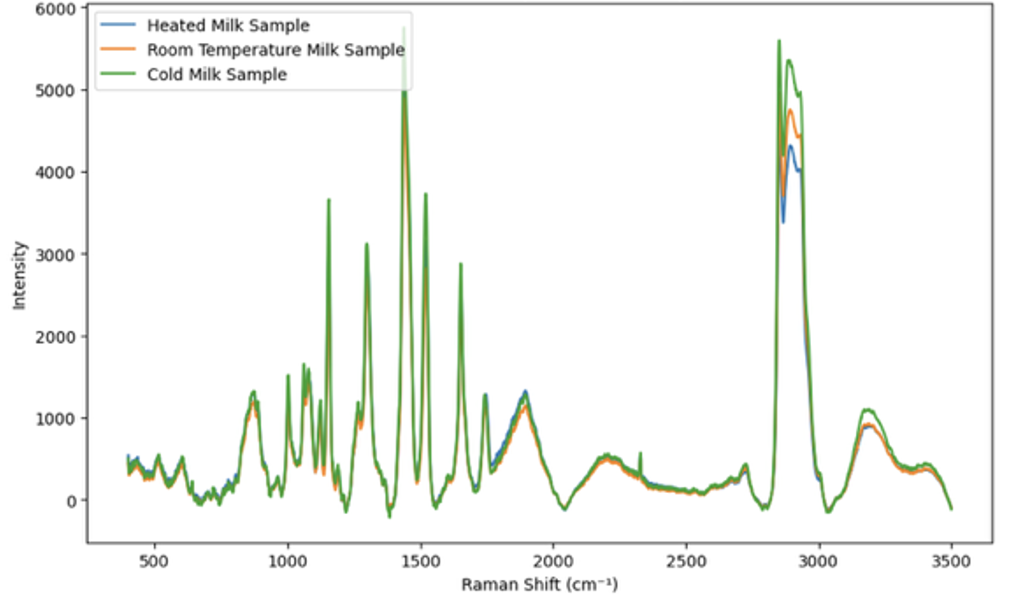
\includegraphics[width=0.5\linewidth]{Figures/Screenshot 2025-07-16 at 2.27.09 PM.png}
    \caption{Variation in Raman Spectra of Control Sample with Temperature}
    \label{fig:temp}
\end{figure}

\begin{figure}[h!]
    \centering
    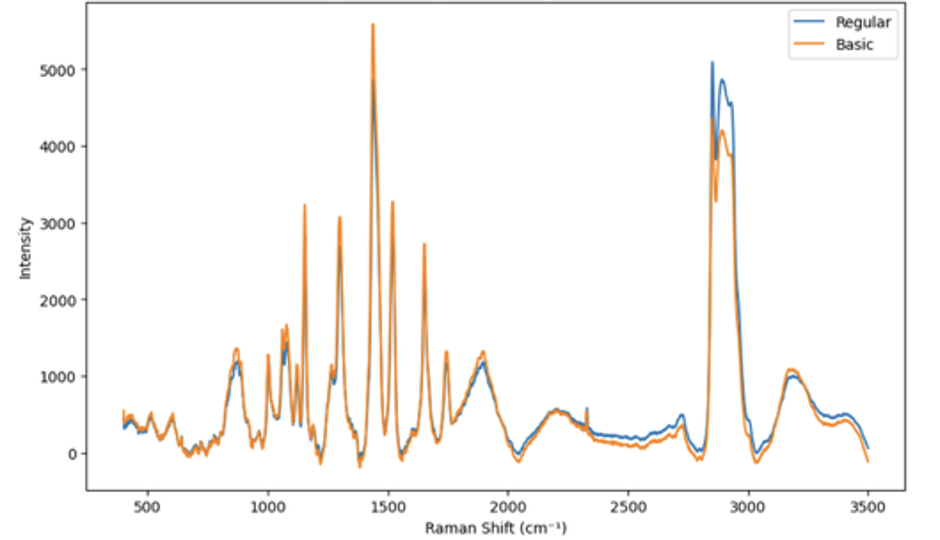
\includegraphics[width=0.5\linewidth]{Figures/Screenshot 2025-07-16 at 2.27.24 PM.png}
    \caption{Variation in Raman Spectra of Control Sample with pH}
    \label{fig:confusion}
\end{figure}

\begin{figure}
    \centering
    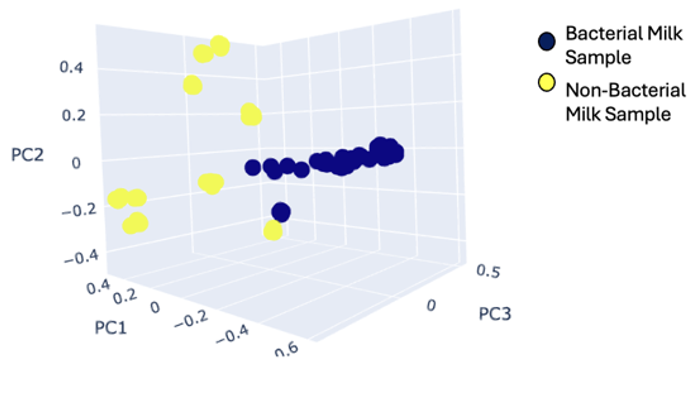
\includegraphics[width=0.5\linewidth]{Figures/Screenshot 2025-07-16 at 2.27.37 PM.png}
    \caption{PCA Analysis of Bacterial and Non-bacterial samples}
    \label{fig:bac}
\end{figure}

\begin{figure}
    \centering
    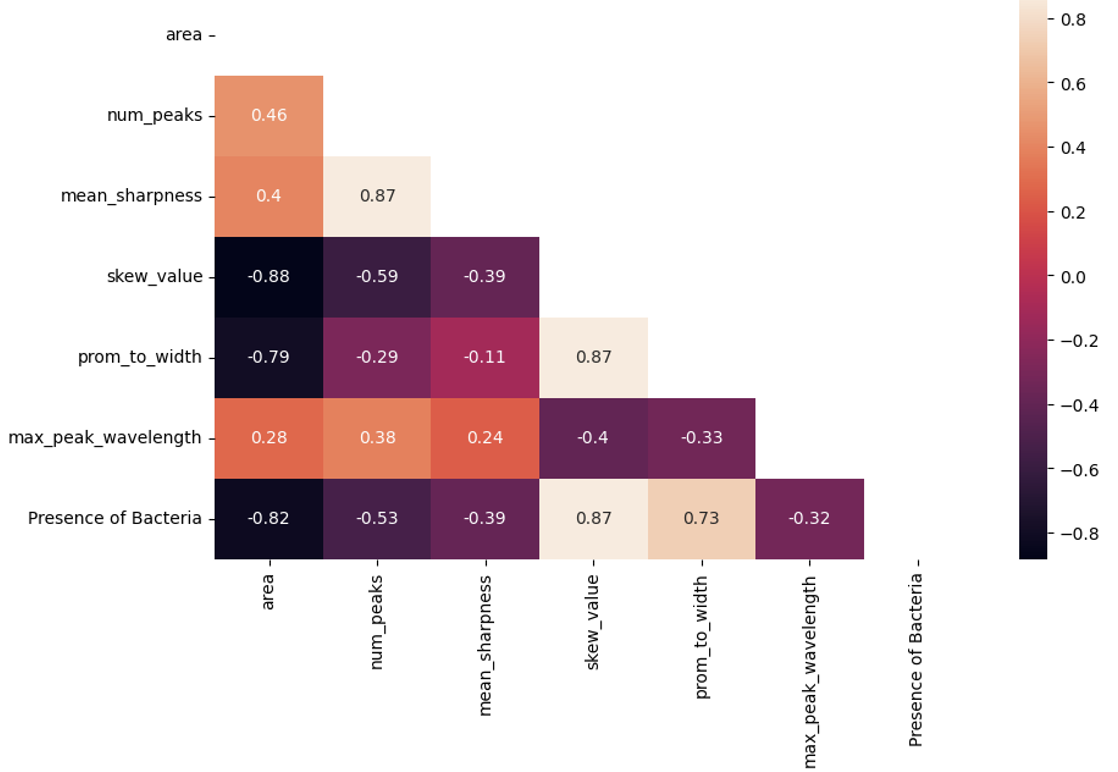
\includegraphics[width=0.5\linewidth]{Figures/Screenshot 2025-07-16 at 2.27.59 PM.png}
    \caption{Correlation Analysis of Feature Extracted Variables}
    \label{fig:corr}
\end{figure}

\begin{figure}
    \centering
    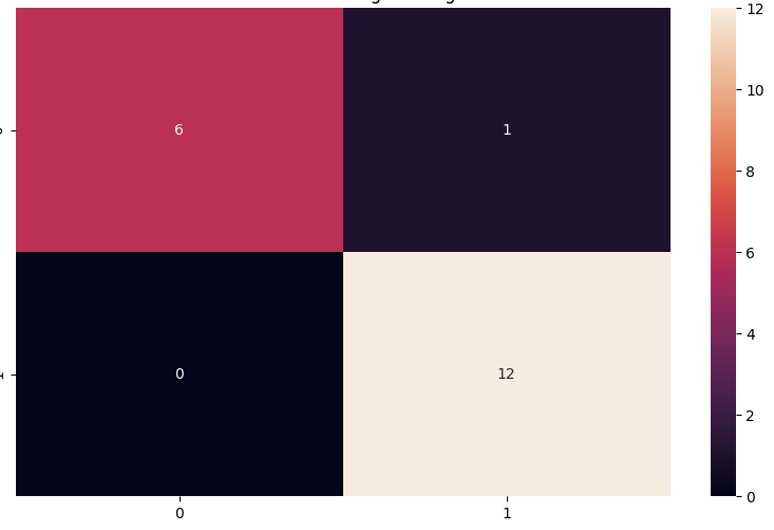
\includegraphics[width=0.5\linewidth]{Figures/Screenshot 2025-07-16 at 2.28.32 PM.png}
    \caption{Confusion Matrix for Logistic Regression, Support Vector Machines and Naive Bayes Classifier}
    \label{fig:cm}
\end{figure}

\begin{figure}
    \centering
    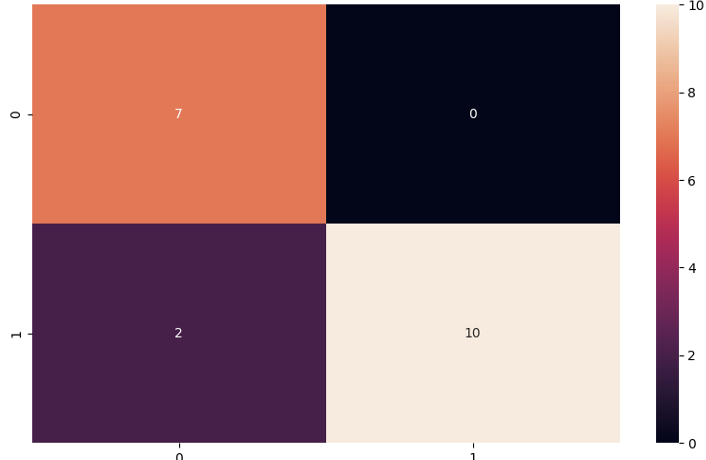
\includegraphics[width=0.5\linewidth]{Figures/Screenshot 2025-07-16 at 2.28.53 PM.png}
    \caption{Confusion Matrix for Gaussian Process Classifiers}
    \label{fig:cm2}
\end{figure}


\end{document}
